%\documentclass[article]{IEEEtran}
\documentclass[final,journal,a4paper]{IEEEtran}

%\IEEEoverridecommandlockouts
% The preceding line is only needed to identify funding in the first footnote. If that is unneeded, please comment it out.
\usepackage[nocompress]{cite}
\usepackage{amsmath,amssymb,amsfonts}
\usepackage{algorithmic}
\usepackage{graphicx}
\usepackage{textcomp}
\usepackage{xcolor}
\usepackage{supertabular,booktabs}
\usepackage{hyperref}
\usepackage[english]{babel}
\usepackage[T1]{fontenc}
\renewcommand\citepunct{, }

\def\BibTeX{{\rm B\kern-.05em{\sc i\kern-.025em b}\kern-.08em T\kern-.1667em\lower.7ex\hbox{E}\kern-.125emX}}
\newcommand{\titel}{Visualizing Uncertainty in Train Delay Predictions: Effects on User Trust, Comprehension, and Decision Quality}
\newcommand{\autorALM}{Anna-Livia Martin}
\newcommand{\autorDR}{David Rossel}
\newcommand{\hochschule}{RheinMain University of Applied Sciences}
\newcommand{\ort}{Wiesbaden, Germany}
\newcommand{\mail}{anna-livia.martin@student.hs-rm.de, david.rossel@student.hs-rm.de}

\begin{document}
% Vorspann
\title{\titel}

\author{
  \begin{minipage}[t]{0.45\textwidth}
    \centering
    \autorALM\\
    \hochschule, \ort\\
    anna-livia.martin@student.hs-rm.de
  \end{minipage}\hfill
  \begin{minipage}[t]{0.45\textwidth}
    \centering
    \autorDR\\
    \hochschule, \ort\\
    david.rossel@student.hs-rm.de
  \end{minipage}
}

\date{\today}

\maketitle

\begin{abstract}
Predictions regarding the probability of train delays can assist travellers in selecting optimal connections, purchasing suitable tickets, and possible compensation claims. However, the question of how such forecasts need to be visualised in practice in order to be comprehensible, credible, and relevant for decision-making by a broad public remains unanswered. As divergent forms of visualisation are subject to differing evaluation in both research and practice, in the paper a user study on forms of uncertainty visualisation was conducted. The objective of this study is to select more effective visualisations for predicting the probability of train delays in practice. The results of this paper show that simple, intuitive visualizations, specifically hybrid representations that combine numerical probabilities with contextual textual explanations and recognisable colour codes (traffic light systems), enhance user understanding, trust, and decision quality. Participants consistently reported greater confidence in their decisions when presented with straightforward, action-oriented visual formats.
\end{abstract}

\begin{IEEEkeywords}
End-user visualization, transit predictions, mobile interfaces, uncertainty visualization, delay predictions, risk communication, user interface design, decision making under uncertainty
\end{IEEEkeywords}

% Content
\section{Introduction} \label{Introduction}
% Hier wird kurz zum Thema eingeleitet. Sobald klar ist um was es geht, wird zu jedem Teil des Papers einmal gesagt was darin erarbeitet wird. 
Rail delay forecasts increasingly appear in journey-planning apps and operator communications, promising to help travellers choose connections, ticket types and, when relevant, to assess potential compensation claims. These forecasts, however, are inherently uncertain: they predict probabilities rather than certainties and often rely on noisy operational data and complex models \cite{Stephenson2003}. For many people, probabilistic information is difficult to interpret \cite{Karagappa2024}; unclear or poorly designed visualisations may reduce the usefulness of the forecasts or even produce misleading decisions. Consequently, the way uncertainty is communicated strongly affects whether predictive systems actually support better decisions \cite{Karagappa2024}. In general, prediction systems often function like black boxes, concealing important details about how recommendations are generated and how they relate to the users context. This is partially because users are often unaware of the underlying considerations, which can undermine trust and effective decision-making \cite{Chatti2024}.
\newline
Two concrete examples of the current state of uncertainty visualisation in delay predictions are the railway apps of Deutsche Bahn \cite{db-webseite} and Rhein-Main-Verkehrsverbund \cite{rmv-webseite}. In both cases delays are only shown as a second time marked in red (see \ref{train-connection-details-db} and \ref{train-connection-overview-rmv}). Neither option provides the possibility to view more detailed information about the uncertainty of the delay forecast, nor is there any further information available. In fact, one could argue that the red delay figures are so small that they could almost be overlooked in comparison to other icons and the design.
\begin{figure}[htbp]
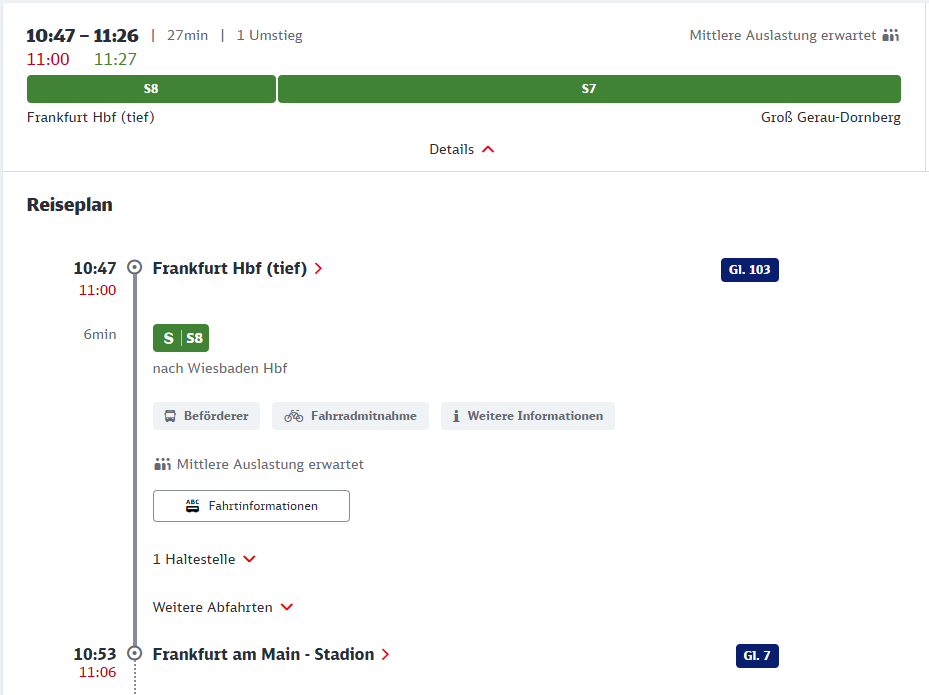
\includegraphics[width=\columnwidth]{Resources/delay-examples-from-reality/train-connection-details-db.png}
\caption{Details of a train connection from the Deutsche Bahn website} \label{train-connection-details-db}
\end{figure}
\begin{figure}[htbp]
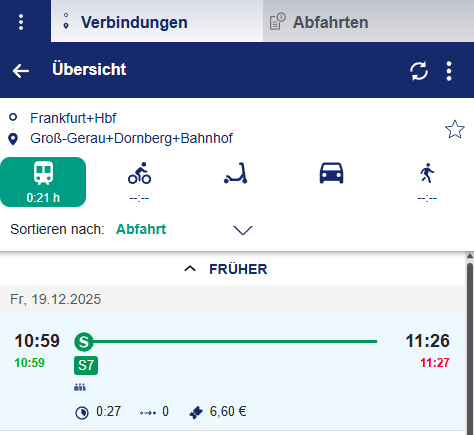
\includegraphics[width=\columnwidth]{Resources/delay-examples-from-reality/train-connection-overview-rmv.png}
\caption{Overview of a train connection from the Rhein-Main-Verkehrsverbund website} \label{train-connection-overview-rmv}
\end{figure}
The uncertainty of this prediction remains completely hidden. This absence of uncertainty information in real-world systems is not accidental. Contemporary data visualization tools provide only limited support and lack established representational standards for conveying uncertainty \cite{Brennen2018}. Passengers must therefore decide whether or not to take the connection without any further information about the likelihood that it will actually arrive on the displayed time. Consider the scenario described by Kay et al. \cite{Kay2016}: the authors present an example in which a person relies on a transit application to decide how to allocate a short time window before a vehicle’s arrival. The application provides a single point estimate for the predicted arrival time. Based on this information, the individual makes a decision that appears reasonable given the displayed estimate. However, the vehicle arrives earlier than indicated, leading to negative consequences. This example illustrates that real-world forecasts are inherently uncertain \cite{Kay2016}. A single numerical prediction does not capture the full range of plausible arrival times. If uncertainty had been communicated more explicitly, by indicating that earlier arrivals were also possible, the decision might have been evaluated differently. The situation is further complicated by well-documented cognitive biases in time estimation. Time-related predictions are frequently subject to systematic underestimation due to optimistic bias, commonly referred to as the planning fallacy. Importantly, this bias persists even when individuals have access to relevant past experience, indicating that informed time estimates are still subject to irrational judgment, explaining why the person in Kay et al.'s \cite{Kay2016} example missed the bus although she might have had similar experiences in the past \cite{Koval2022}. This example illustrates how point estimates can encourage overconfidence in predictions and lead to suboptimal decisions. 
\newline
Concrete examples of public-facing uncertainty visualisations can be found in journalism. The New York Times has used simulation-generated samples to illustrate uncertainty in employment projections and potential outcomes of political elections to general audiences \cite{nytimes, nytimes-whowillwin}. Similarly, the Wall Street Journal highlighted how numerical presentations can mislead readers \cite{Ellenberg2015}. These examples demonstrate that even widely consumed forecasts often struggle with effectively conveying uncertainty, reinforcing the importance of carefully designed visualisations that make probabilistic information interpretable to non-experts. Same could be argued for the authors of scientific papers. Masen et al. \cite{Mason2024} argue that authors operate in a field of tension: on the one hand, omitting representations of uncertainty is considered scientifically problematic or even misleading; on the other hand, many authors avoid precisely these representations out of concern that their results might appear less credible as a result \cite{Mason2024}. This tension highlights the negative consequences of focusing on trust rather than transparency \cite{Mason2024}. Particularly in cases of high uncertainty, researchers tend to omit relevant information because it could weaken confidence in their conclusions \cite{Mason2024}. This is a direct consequence of focusing uncertainty visualisations primarily on increasing trust rather than on honest disclosure of uncertainty \cite{Mason2024}.
\newline
Explicitly visualizing uncertainty, in contrast, can improve long-term user trust and decision quality, whereas reliance on point estimates often results in systematic decision errors \cite{Kay2016}. Beyond conveying probabilistic values alone, prior work emphasizes that effective uncertainty visualizations must also provide contextual information to support risk assessment. Visualizations should therefore communicate relationships between risks, underlying assumptions, possible scenarios, and mitigation strategies in order to enable informed decision-making \cite{Dikmen2024}. This is often times made difficult because of the potentially overwhelming amount of output data. Controlling the ``explosion'' of information is critical to avoid overloading users while still conveying the relevant probabilistic and contextual information \cite{GrietheSchumann}. %Furthermore, providing uncertainty information influences the way humans integrate multiple sources of conflicting information. People do not simply average different inputs, but weigh each according to its reliability. Moreover, the amount of uncertainty information included in a visualization shapes the internal models people use to combine information \cite{Greis2018}.
\newline
Providing additional explanatory information can substantially improve user performance and subjective outcomes without increasing cognitive burden \cite{Yang2020, Chung2020, Chakraborty2025}. Adding explanations increases task success, reduces the number of trials required to achieve success, and improves user comprehension and confidence, while not increasing perceived task load \cite{Chakraborty2025}. Similarly, Bansal et al. \cite{Bansal2021} found that access to explanations made people more inclined to accept the suggestion, regardless of its accuracy or the persons own expertise. This suggests that displaying uncertainty of predictions could contribute to positive chronotation not only from the perspective of travellers, i.e. the users of the transit app, but also from the perspective of the transport companies.
\newline
The communication and visualization of uncertainty is an active research topic addressed by a broad, interdisciplinary community \cite{Skeels2008}. Relevant contributions span psychology \cite{Jenkins2020}, multiple areas of computer science, including human-computer interaction and visualization \cite{Inkpen2023, Dong2024}, as well as design research \cite{Kay2016}, geographical visualisation and geoinformation science \cite{Skeels2008}. However, there are only a few studies that specifically address the representation of uncertainty for non-expert target groups \cite{Kay2016}. Given the inherent complexity of uncertainty information, prior work has argued that the evaluation of uncertainty visualizations should focus less on identifying a single “best” representation and more on whether a visualization effectively supports users in accomplishing their tasks. The central question should be “does it help,” rather than “which visualization is better” \cite{Harrower}. Therefore, the overarching objective of uncertainty visualization is the seamless integration of uncertainty information into the data presentation itself, rather than treating it as an add-on \cite{Potter2010visualizationofuncertainty}. Despite numerous proposed approaches, a comprehensive discussion of their effectiveness across contexts remains scarce, as corresponding usability studies are still relatively rare \cite{GrietheSchumann}. This gap motivates an investigation into uncertainty visualizations specifically for everyday decision-making in the context of train delays. The study aims to contribute to a better understanding of possible uncertainty visualisations for predictions in the context of everyday decision-making, specifically evaluating which forms of visualisation increase confidence in predictions and reduce erroneous decisions and further understanding in relation to such predictions.
\newline
\newline
The papers three contributions are: 
\begin{enumerate}
    \item eliciting domain-specific design requirements and a nuanced description of user needs for visualising uncertainty in train-delay predictions, based on two rounds of expert interviews;
    \item proposing design layouts for various forms of uncertainty visualisation to display train arrival times on small smartphone screens; and
    \item evaluating the visualisations in a user study combining quantitative measures and qualitative interviews, reporting comparative effects on perceived trust, understanding and decision quality, and deriving practical design guidelines for journey-planning applications
\end{enumerate}
Section \ref{Background and Related Work} provides an overview of the state-of-the-art in uncertainty visualization and risk communication. Section \ref{Research Questions and Hypotheses} then formulates the research questions and hypotheses. Section \ref{Expert Study} describes the implementation and evaluation of the expert interviews. Based on the results of the interviews, \ref{Design of Wireframes} outlines the wireframes used to represent uncertainty predictions for selected visualizations. Section \ref{User Study} describes the implementation and evaluation of the user study. This is followed by a discussion of the results in \ref{Discussion}. Finally, possible limitations and further research opportunities are listed in \ref{Limitations and Future Work}, followed by a conclusion in \ref{Conclusion}.

\section{Background and Related Work} \label{Background and Related Work}
Numerous studies have already dealt with the visualisation of uncertainties in forecasts. In the following section, these approaches are systematically presented and distinguished from one another. The general aim of visualising uncertainty is to reduce misinterpretations \cite{Kamal2021}. Therefore, uncertainty data should be presented as accurately as possible \cite{Kamal2021}, because ``[f]ailing to observe [uncertainty] in visualization can lead to flawed decision-making'' \cite{Kamal2021}. At the same time, the form of visualisation is influenced by the quality and volume of uncertain data, the lack of complete certainty in the data, and the perceptual and cognitive confusion caused by the representation itself \cite{Jena2020}. It is therefore necessary to find a form of visualisation that represents uncertainty as accurately as possible while at the same time avoiding misinterpretation by the analyst.

\subsection{Dependence on the users skills} \label{Dependence on the user's skills}
%``While these systems are powerful, they do make mistakes occasionally, leading to misuse. Sometimes these systems are underestimated by people, leading to disuse.'' \cite{Parasuraman1997} ``Both disuse and misuse could cause serious problems'' \cite{Marsh2005}
One of the earliest works by Covello et al. \cite{Covello1988} states that problems in risk communication are caused, among other things, by a lack of understanding of scientific methods, models and data. This is supported by further studies. Jena et al. \cite{Jena2020} note that while there is limited empirical evidence on how analysts and non-experts process and interpret different forms of visualisation of uncertainty, the effectiveness of visualisation depends on the relative spatial and numeracy ability of the individual. Beyond general perceptual and numeracy skills, prior work indicates that many existing approaches implicitly assume substantial technical expertise on the user side. Much of the existing research has focused on explaining the underlying algorithmic mechanisms \cite{Liu2018}, thereby presuming that users possess advanced knowledge of machine learning concepts \cite{Liu2018}. However, end users are often domain experts who do not necessarily have the background required to understand how such algorithms operate, or in this papers example, they may be non-experts with no prior knowledge of graphics. This mismatch between designers’ assumptions and users’ actual expertise has been identified as a potential cause of recent controversial and counter-intuitive findings, such as evidence suggesting that explanations can even be harmful \cite{Stumpf2018}. Visualisations can help analysts better understand classifications by increasing the transparency of the model \cite{Yuan2021SurveyVisAnalyt}. Although explanations have a positive effect, empirical studies indicate that the understanding of conditional probabilities by experts and non-experts is limited, regardless of the representation \cite {Eddy1982, Tversky2013, Gigerenzer1995, Weber2018}. For example, Belia et al. \cite{Belia2005} showed that even experts make mistakes when interpreting error bars \cite{Belia2005} and even people with good basic statistical knowledge underperformed when interpreting graphics of uncertain quantities \cite{Ibrekk1987}. In response to this, studies are increasingly using other static, abstract representations of distributions (e.g. box plots, violin plots, gradient plots) \cite{Potter2010SummaryStatistics}. Correll et al. \cite{Correll2014} note here that these are often more expressive of the distribution and can avoid biases associated with reading error bars. Nonetheless, if people have less static prior knowledge, it is more difficult for them to understand this uncertainty through statistical visualisation \cite{Greis2017}. Spiegelhalter et al. \cite{Spiegelhalter2011} therefore recommend assuming limited numerical competence on the part of a general audience when designing forms of visualisation. Specifically, a ``less is more'' approach is proposed, which minimises the need for complex conclusions, presents comparisons clearly and explicitly, and makes additional detailed information optionally accessible \cite{Spiegelhalter2011}. This is supported by Thomas et al. \cite{Thomas2024}, who compared six visualisations and found that visualisations with more details led to worse performance and Greis et al. \cite{Greis2015}, who found that ``familiarity, easiness to understand, and visual appeal'' have a massiv influence on the unterstanding. We therefore argue that visualisations for representing uncertainty do not necessarily need to expose large amounts of detailed information. Instead, the primary objective should be to support user understanding and to promote appropriate decision-making. This perspective aligns with Correll et al.’s \cite{Correll2014} argument that visual encodings should encourage “the right behavior” from viewers even when users lack statistical (or graphical) training.
\newline
This emphasis on promoting appropriate user behavior is further supported by findings on how people conceptualise and communicate uncertainty. Skeels et al. \cite{Skeels2008} found that many participants expressed uncertainty using qualitative, non-standardised categories rather than precise numerical values, often relying on informal constructs such as “small,” “medium,” or “large”. These representations were typically created within a group and rarely stored explicitly with the data. Such findings closely align with the idea of using simplified categorical encodings, for example traffic-light-style representations, to communicate uncertainty \cite{Skeels2008}. Interestingly, when asked how uncertainty should be visualised, participants most frequently referred to familiar statistical representations, in particular error bars, despite their previously expressed qualitative understanding of uncertainty \cite{Skeels2008}. This reveals a gap between users’ internal conceptualisations of uncertainty and the visual encodings they are accustomed to, which may contribute to misinterpretation and overconfidence. Beyond representational familiarity, cognitive factors further influence the effectiveness of uncertainty visualisations. Bancilhon et al. \cite{Bancilhon2023} showed that individuals with low working memory capacity made fewer errors and experienced lower subjective workload when uncertainty was conveyed through visual encodings such as icon arrays rather than text alone. This suggests that appropriately designed visualisations can improve decision accuracy while simultaneously reducing cognitive demand. Taken together, these findings reinforce the argument that no single visualisation is universally optimal. Prior work has emphasised that different graphical representations serve different communicative functions and that their effectiveness varies across contexts and user groups \cite{Lipkus1999, Spiegelhalter2011, Spiegelhalter2017}. Consequently, Spiegelhalter et al. \cite{Spiegelhalter2011} argue that designing uncertainty visualisations should begin with a systematic analysis of the target audience and their needs, followed by an iterative process of design, evaluation, and refinement to arrive at an appropriate final representation.

\subsection{Assessment techniques for decision-making} \label{Assessment techniques for decision-making}
% Wie genau lassen sich Visualisierungsformen für Unsicherheit systematisch bewerten und entlang welcher Dimensionen?
As pointed out in \ref{Dependence on the user's skills}, visualisations should not be evaluated based on how much information they display, but rather on whether they support appropriate decision-making behaviour under uncertainty. Uncertainty is a multifaceted concept for which no universally accepted definition exists \cite{GrietheSchumann}. Rather than representing a single, well-defined quantity, uncertainty has been described as a composition of different aspects, including error, imprecision, accuracy, lineage, subjectivity, non-specificity, and noise \cite{GrietheSchumann}. These aspects can originate from various sources throughout the data lifecycle, arising during data acquisition, processing, modelling, or visual representation \cite{GrietheSchumann}. As a result, uncertainty visualisations must account for heterogeneous uncertainty sources and characteristics, which complicates both their design and their evaluation. Consequently, assessing uncertainty visualisations requires a multidimensional perspective that goes beyond a single definition or metric and instead considers how different forms of uncertainty are communicated and interpreted in decision-making contexts. To assess uncertainty visualisations in the context of decision-making, prior work suggests that no single metric is sufficient \cite{Langer2022, Brennen2018}. Instead, evaluation must account for cognitive, behavioural, and perceptual factors, as well as different forms of uncertainty. Building on existing literature, the assessment techniques are structured along four complementary dimensions: cognitive load, decision behaviour, uncertainty perception, and transparency.

\subsubsection{Cognitive Load and Information Processing}
Cognitive Load is a central dimension for assessing uncertainty visualisations, as human working memory capacity is limited and easily overwhelmed by complexity. Prior work has therefore employed both subjective and behavioural measures to evaluate how visual representations affect information processing. For instance, Langer et al. \cite{Langer2022} assess the impact of terminology using metrics such as trust, perceived complexity, controllability, and familiarity. Brennen et al. \cite{Brennen2018} further propose reported confidence and cognitive load as key evaluation criteria for uncertainty visualisations \cite{Brennen2018}. These approaches are grounded in Cognitive Load Theory, which distinguishes between intrinsic load-determined by the inherent difficulty of a task relative to a user’s prior knowledge and extraneous load, which arises from representational or instructional features that do not contribute to learning or understanding \cite{Paas2010}. From this perspective, uncertainty visualisations should aim to minimise extraneous cognitive load while preserving task-relevant information. Empirical evidence suggests that visual encodings can substantially influence both cognitive load and comprehension. Fritz et al. \cite{Fritz2025} demonstrate that different visualisation forms significantly affect pilots’ cognitive load and understanding in operational contexts \cite{Fritz2025}. We argue that these findings are transferable to uncertainty visualisations for forecasting tasks, where inappropriate visual complexity may similarly impair interpretation and decision-making.

\subsubsection{Decision Behaviour and Decision Adaptation}
Beyond cognitive processing, uncertainty visualisations must be evaluated based on their influence on users’ actual decision behaviour. Reyes et al. \cite{Reyes2025} investigate visual encodings of AI uncertainty using size, colour saturation, and transparency, introducing metrics such as decision change, trust, and perceived decision certainty \cite{Reyes2025}. Decision change captures whether users revise their choices when exposed to different uncertainty representations and thus serves as a behavioural indicator of how visualisations affect decision-making. Prior research highlights the importance of distinguishing between self-reported and behavioural measures. Papenmeier et al. \cite{Papenmeier2022} define self-reported trust as questionnaire-based, reflective assessments, whereas behavioural trust is inferred from observable actions, such as reliance or switching behaviour. Their findings show that self-reported trust and behavioural indicators, such as switching rates, do not necessarily align, complicating the evaluation of trust in automated decision-making systems.
\newline
These results suggest that decision-related metrics, including decision change and switching behaviour, provide more robust insights into how uncertainty visualisations shape user behaviour than subjective confidence ratings alone. Consequently, effective assessment should focus on whether visualisations encourage appropriate adjustments of decisions in response to uncertainty, rather than merely increasing perceived certainty or trust.

\subsubsection{Representing Risk, Uncertainty, and Ambiguity}
Assessing uncertainty visualisations further requires accounting for different forms of uncertainty and their implications for decision-making. In economics and the social sciences, a common distinction is drawn between risk-situations with agreed quantification based on extensive data and uncertainties, where such quantification is not possible \cite{Spiegelhalter2017}. This distinction is often extended to include ignorance, referring to unknown or unknowable factors \cite{Spiegelhalter2017}. In addition, the concept of ambiguity is used inconsistently across disciplines, as denoted by Spiegelhalter et al. \cite{Spiegelhalter2017}. In behavioural economics, ambiguity typically denotes uncertainty about probabilities, whereas other interpretations refer to contested or unknown outcomes or values \cite{Spiegelhalter2017}. These distinctions are relevant for evaluation, as different visualisations may be suitable for different uncertainty types and communicative goals. From a risk communication perspective, effectiveness is not defined by completeness alone but by whether a representation contributes to the intended decision outcomes \cite{Spiegelhalter2017}. 
\newline
Accordingly, uncertainty visualisations should be assessed based on their ability to make the nature and limits of available knowledge explicit, to support appropriate caution, and to discourage unwarranted precision or overconfidence in situations characterised by uncertainty or ignorance.

\subsubsection{Transparency, Interpretability, and Explanation}
Transparency, interpretability, and explanation are closely related but distinct concepts in the evaluation of uncertainty visualisations. Papenmeier et al. \cite{Papenmeier2022} define transparency as the extent to which information about a system’s inner workings is exposed, whereas interpretability refers to the degree to which this information is meaningful to a human user \cite{Papenmeier2022}. Explanations are understood as the mechanisms through which transparency is communicated to users \cite{Papenmeier2022}. A substantial body of work suggests that explanations can positively influence trust and transparency, particularly when they are visual or verbal \cite{Kizilcec2016, Dasgupta2017, Wang2016}. Richer explanations have been associated with higher trust and improved performance \cite{Yang2020, Zhang2020}. However, recent studies also indicate that the type of transparency provided affects trust \cite{Ghai2021, Zhang2020}. These studies therefore strengthen the explainability-trust thesis, which suggests that ``Explainability is a suitable means for facilitating trust in a stakeholder'' \cite{Sadeghi2024, Kastner2021}. There are many different definitions of trust in the literature \cite{Reyes2025, Watson2005, McKnight2001}. We define trust according to the definition Madsen et al. \cite{Madsen2000} uses, which is derived from McAllister et al., trust describes ``the extent to which a user is confident in, and willing to act on the basis of, the recommendations, actions, and decisions of an artificially intelligent decision aid''.
\newline
It is widely believed that explaining how a system works increases user confidence in the system \cite{Elofson2001, Glass2008, Pu2006, Wang2007} and reduces aversion to a system \cite{Dietvorst2015}. Studies found that users only used automation when they trusted the system more than themselves \cite{Muir1996, Barredo2020}. Trust and risk perception are particularly important in forecast-based systems \cite{Kenesei2025}. User acceptance and trust in AI systems depends heavily on how understandable the systems capabilities and explanations are \cite{Druce2021, Bahlmann2014}. Whereby visual explanations generally have a positive effect on transparency \cite{Ma2021}. We argue that trust in uncertainty visualisations for predictions is equally important, because without trust, there will be no use of the prediction. Therefore, as Kastner et al. \cite{Kastner2021} denote ``trustworthiness is a property worth engineering towards'' when displaying uncertainties of predictions.

\subsection{Visualisation Techniques}
Visualising uncertainty is a central task in decision-making contexts, as it enables users to interpret predictions, assess risks, and make informed choices. Various techniques have been proposed in the literature, ranging from simple error bars to complex probabilistic displays and hybrid textual-graphical representations \cite{Kay2016, GrietheSchumann, Potter2012}.

To provide a structured overview, Table~\ref{tab:visualisations} summarises the visualisation forms considered in prior studies. The table indicates both the type of representation and the studies in which it has been empirically investigated. This overview serves two purposes: first, it highlights the diversity of approaches explored in the literature; second, it informs the selection of visualisations for comparative evaluation in the context of this work. As such, the visualisations included are not exhaustive but represent a set of commonly studied and practically relevant techniques.
\begin{table}[htbp]
\centering
\caption{Overview of visualisation forms and corresponding studies} \label{tab:visualisations}
\tablefirsthead{
\toprule
Visualisation Form & Count & Studies \\
\midrule
}
\tablehead{
\multicolumn{3}{c}{{\bfseries Continued from previous column}} \\
\toprule
Visualisation Form & Count & Studies \\
\midrule
}
\tabletail{
\midrule
\multicolumn{3}{r}{{Continued on next column}} \\
\midrule
}
\tablelasttail{
\midrule
\multicolumn{3}{r}{{Concluded}} \\
\bottomrule
}
\tabletail{
\midrule
\multicolumn{3}{r}{{Continued on next column}} \\
\midrule
}
\begin{supertabular}{p{3.5cm} p{1cm} p{3cm}}
Error bars / Bar chart & 9 & \cite{Thomas2024, Dikmen2024, Ibrekk1987, Hullman2015, Hgele2022, Chatti2024, Skeels2008, Greis2015, Kay2016} \\
Box plot & 6 & \cite{Brennen2018, Correll2014, Ibrekk1987, Potter2010visualizationofuncertainty, Chatti2024, Skeels2008} \\
Gradient plot & 3 & \cite{Brennen2018, Correll2014, Tak2014} \\
50-dot quantile plot & 3 & \cite{Koval2022, Kay2016, Greis2018} \\
Line chart & 3 & \cite{Koval2022, Chatti2024, Greis2015} \\
Numerical expression & 2 & \cite{Thomas2024, Jenkins2020} \\
Pie chart & 2 & \cite{Ibrekk1987, Chatti2024} \\
%Violin plot & 2 & \cite{Correll2014, Hullman2015} \\
%scatter plot & 2 & \cite{Brennen2018, Chatti2024} \\
Functions & 2 & \cite{Ibrekk1987, Kay2016, Greis2015} \\
Stacked bar chart & 2 & \cite{Chatti2024, Greis2015} \\
%spaghetti plot & 2 & \cite{Tak2014, Potter2010visualizationofuncertainty} \\
%rose chart / polar area chart & 2 & \cite{Yang2020, Chatti2024} \\
Textual representation & 1 & \cite{Greis2015} \\
\end{supertabular}
\end{table}

\subsubsection{Error Bars}
Error bars commonly represent uncertainty around central estimates but often lead to underweighting and perceptual biases \cite{Hullman2015, Correll2014, Newman2012}. Correct interpretation requires statistical experience \cite{Belia2005}, though symmetric encodings around the mean mitigate some biases \cite{Correll2014}. Despite limitations, error bars remain popular due to familiarity \cite{Skeels2008}.

\subsubsection{Box Plots}
Box plots summarise distributions by visualising median, quartiles, and outliers. They offer a compact overview of central tendency and spread, making them suitable for comparing multiple categories \cite{Chatti2024}. Ibrekk et al. \cite{Ibrekk1987} show that box plots and error bars perform well for illustrating means but are less effective for probability intervals with non-uniform densities \cite{Ibrekk1987}.

\subsubsection{Gradient Plots}
Gradient plots encode uncertainty via transparency or colour intensity variations, presenting it as a continuous field. Correll et al. \cite{Correll2014} propose them as superior to bar charts with error bars for inferential tasks, reducing perceptual biases. Tak et al. \cite{Tak2014} confirm good performance for normally distributed data, though display conditions can affect interpretability.

\subsubsection{50-dot Quantile Plot}
50-dot quantile plots represent discrete outcomes and improve precision via subitizing by counting individual marks \cite{Kay2016}. Excessive dots cause density-like perceptions and variance overestimation. They suit small-to-moderate datasets but require careful design to avoid visual clutter \cite{Kay2016}.

\subsubsection{Numerical Expression}
Numerical formats (probabilities, percentages, standard deviations) effectively communicate uncertainty \cite{GrietheSchumann}. Jenkins shows numerical intervals outperform verbal formats, reducing extremity effects and maintaining communicator credibility even when wrong \cite{Jenkins2020}. Graphics convey message essence, while numbers explain details; numerical annotations on graphical elements are common \cite{Feldman-Stewart2007, Spiegelhalter2017, Kay2016}.

\subsubsection{Pie Chart}
Pie charts were used early for proportions and probabilities but are problematic for uncertainty visualisation \cite{Ibrekk1987}. They initially enable good probability estimation but performance declines with deliberate reasoning, suggesting fragile intuitive interpretations \cite{Ibrekk1987}.

\subsubsection{Textual representation}
Textual explanations provide additional context or guidance for decision-making. In human-AI collaboration, clear action recommendations have been shown to improve decisions for novice users with limited domain knowledge \cite{Inkpen2023, Dong2024}. Similar results were observed by Koval et al. \cite{Koval2022} with interactive texte improving decision making. However, overly complex explanations can be counterproductive if they assume knowledge the user does not possess \cite{Krause2018}. Simplified technical language, contextual definitions, and standardized terminology are recommended to enhance comprehension \cite{Jit2025}. Textual annotations can complement visualisations but should be used sparingly to avoid cognitive overload \cite{Chen2025}. Another study examined how the visual design of severe weather forecasts can influence communication and decision-making. It found that external forms of uncertainty representation that incorporate additional elements such as explanatory text can help to interpret probabilities more accurately. Internal representations, on the other hand, which alter existing graphic variables such as colour intensity, are less effective in supporting correct interpretations \cite{Clive2023}. Contrary to this trend, Al-Taie et al. \cite{Al-Taie2014} found that human eyes can interpret graphs faster than texts because different visual elements are recognized simultaneously. This could indicate that texts lead to a higher cognitive load than graphics \cite{Al-Taie2014}.
\newline
Several earlier studies combine text and graphics. The results suggest that their combination might provide learning benefits instead of showing only one of them \cite{Bruny2008, Bruny2006}. Jenkins examines how different formats of communicating uncertainty (verbal, numerical, mixed) are understood by non-experts and how they influence the perceived credibility of the communicator \cite{Jenkins2020}. It becomes clear that mixed verbal-numerical formats (e.g. ``unlikely [20\%]'') and numerical-verbal formats (``20\% [unlikely]'') can improve understanding \cite{Jenkins2020}.

\subsubsection{Traffic Light System}
Traffic-light encodings (red/yellow/green) or qualitative labels (low/moderate/high) communicate uncertainty simply and accessibly \cite{Potter2012, Skeels2008, Clive2023}. Participants prefer adjacent displays with clear signals \cite{Potter2012}, and vertical ``risk ladders'' aid probability understanding with action guidance \cite{Lipkus1999}. Color-coded signals work well in AI and safety-critical contexts \cite{Dong2024, Yu2025}. Skeels et al. \cite{Skeels2008} found participants used non-standardized qualitative labels like ``t-shirt sizes'' internally, aligning with traffic light concepts.

\subsubsection{Functions, Distribution and Line Charts}
Line charts with shaded confidence intervals improve decision accuracy, particularly for timing tasks like train connections \cite{Koval2022}. Probability density functions and histograms provide complete uncertainty views but require statistical literacy \cite{Greis2015, Belia2005}. Users prefer function graphs despite limited intuition, though excessive detail may not enhance decisions \cite{Greis2015}.

\subsection{Issues with Visualization}
Despite the wide range of proposed techniques for visualizing uncertainty, prior work has repeatedly highlighted fundamental challenges that can undermine user understanding, trust, and decision quality. Al-Taie et al. \cite{Al-Taie2014} identify clutter, excessive detail, and increasing time complexity as central problems in information visualization, particularly when multiple uncertainty cues are displayed simultaneously. Such overload can obscure relevant signals and place unnecessary cognitive demands on users, ultimately reducing the effectiveness of the visualization. Beyond perceptual overload, uncertainty visualizations face the challenge of balancing informativeness with interpretability. Mason et al. \cite{Mason2024} argue that effective uncertainty visualizations should emphasize meaningful and well-justified signals in order to support trust in the results, while simultaneously suppressing information that is dominated by noise. If noisy or weak signals are visually overemphasized, users may draw unjustified conclusions or develop false confidence in uncertain predictions. Another related problem concerns the communication of limitations. Spiegelhalter et al. \cite{Spiegelhalter2011} stress that visualizations should clearly convey the boundaries of the information they present, both in terms of data quality and relevance. Visual representations inevitably simplify complex underlying processes and can only depict a partial view of a broader context. When these limitations are not made explicit, users may overgeneralize from the visualization or misinterpret its scope, leading to misplaced trust or inappropriate decisions. In addition to graphical design, textual elements accompanying visualizations introduce further challenges. Langer et al. \cite{Langer2022} demonstrate that terminology such as ``algorithm'' or ``AI'' is not a neutral design choice but shapes perceptions of complexity, controllability, familiarity, and competence. Their results show that higher technical affinity is associated with higher perceived competence and lower perceived complexity, whereas abstract or technical labels tend to reduce familiarity and trust. This implies that the wording used in textual explanations can act as a mediator between representation and trust. We assume that these effects are transferable to visualizations of uncertainty: visual designs that appear overly technical, abstract, or opaque may increase perceived complexity and reduce trust, while simpler, more familiar representations may foster a sense of understanding and control.

\section{Research Questions and Hypotheses} \label{Research Questions and Hypotheses}
The preceding sections have shown that the visualization of uncertainty is a well-established yet unresolved research problem. Prior work has proposed a wide range of visual encodings and assessment criteria, highlighting trade-offs between precision, interpretability, cognitive load, and trust. At the same time, empirical evidence remains fragmented, context-dependent, and often focused on expert users or abstract tasks. In particular, comparatively little is known about how different uncertainty visualizations affect non-expert users in everyday decision-making situations, such as assessing potential train delays in long-distance rail travel.
\newline
At the beginning of the project, an initial assumption about potential users was formulated to guide the early design process and the development of the research questions. While the system is conceptually intended to be usable by a broad range of travellers, young people in higher education or vocational training are considered a particularly relevant user group, as they frequently rely on public transport and digital travel-planning tools. This assumption served as a starting point for framing the research questions and preparing the subsequent expert interviews.
\newline
This work therefore aims to complement existing research by investigating how different visual representations of uncertain delay predictions influence user trust, understanding, and decision quality in a realistic application context. Based on the reviewed literature, parts of this investigation are already informed by existing findings. In particular, the question of which visualization techniques have been proposed for communicating risk and uncertainty, as well as which evaluation metrics are commonly employed, has been addressed in the related work section. Building on this foundation, the present study focuses on empirically comparing selected visualization forms within a concrete usage scenario and analysing their effects on user behaviour and perception. Accordingly, we formulate the following main research question:

\begin{quote}
\hypertarget{rq:1}{}\textbf{RQ1:} How do different visualizations of uncertain train delay predictions affect users’ trust, understanding, and decision quality in the context of long-distance rail travel?
\end{quote}

To operationalize this question, we further define the following sub-questions:

\begin{itemize}
    \item \hypertarget{rq:1.1}{}\textbf{RQ1.1:} How do different visualization forms differ with respect to perceived comprehensibility, cognitive load, decision quality, and perceived trustworthiness?
    \item \hypertarget{rq:1.2}{}\textbf{RQ1.2:} Which visual design characteristics contribute to increased or decreased user trust in uncertain delay predictions?
    \item \hypertarget{rq:1.3}{}\textbf{RQ1.3:} Which visualization forms best support users in making decisions related to potential compensation claims in cases of predicted delays?
\end{itemize}

In addition to these exploratory research questions, this study tests a set of theory-driven hypotheses derived from prior findings in \ref{Background and Related Work}. These hypotheses focus on the role of abstraction level, categorical encoding, and explanatory context in shaping user trust and understanding.

\begin{quote}
\hypertarget{h:1.1}{}\textbf{H1.1:} Simple, categorical visualizations like traffic lights systems or qualitative labels are perceived as less trustworthy than numerical probability representations but are better understood. Visualizations that include complex graphs are less well understood by users but do not necessarily increase perceived trust.
\end{quote}

\begin{quote}
\hypertarget{h:1.2}{}\textbf{H1.2:} Users prefer visualisations that provide a clear, interpretable statement or implicit instructions for action (e.g. ``high risk'' or ``low risk'') over representations that require interpretation.
\end{quote}

\begin{quote}
\hypertarget{h:1.3}{}\textbf{H1.3:} A brief textual explanation accompanied by a traffic light-style visualisation increases confidence in the prediction and is the preferred option for prompting decisions. It contains both implicit instructions for action and an explanation of how to use it, which leads to fewer incorrect decisions when selecting a train.
\end{quote}

\section{Expert Study} \label{Expert Study}
To identify suitable visualizations and metrics addressing research questions \hyperlink{rq:1.1}{1.1} and \hyperlink{rq:1.1}{1.2}, we conducted a comprehensive literature analysis complemented by iterative expert interviews with UI/UX and human-computer interaction specialists. This preliminary selection process laid the foundation for subsequent empirical validation through a user study.

\subsection{Planning Expert Interviews}
We employed semi-structured guided interviews to pre-evaluate visualizations identified from literature for their usability within the specific use case of Kay et al.'s \cite{Kay2016} train delay scenario. Following established methodological standards \cite{Blasius2019, Kleemann2013}, the questionnaire incorporated open-ended questions alongside narrative prompts designed to elicit comprehensive responses, systematically assessing both visualization effectiveness and appropriate evaluation metrics.

The visualisations were deliberately selected based on their prevalence in the existing literature in conjunction with the hypotheses of the studies, such as the traffic light system. This selection represented a balance between frequently documented approaches, including those subject to methodological criticism, such as error bars, while deliberately avoiding visual redundancy (e.g. by limiting the display to one type of diagram per function category, such as line diagrams or 50-point diagrams). The use of greyscale eliminated the distortion caused by colours as a confounding variable.

The interview process was iterative, consisting of two distinct phases structured as design sprints. The first round involved data collection, immediate analysis and presentation of the results, followed by targeted revision of both the questionnaires and the visualisation stimuli in line with the experts preferences. In a second round, a new group of experts was then interviewed using the optimised materials, enabling immediate analysis and synthesis after the interview.

\subsection{Rationale for the Selection of Visualisation Forms}
Eight visualisation forms (stacked bar chart, box plot, gradient plot, numerical statement, 50-dot quantile plot, pie chart, textual representation, traffic light system) were selected to systematically compare distinct representational strategies for communicating uncertainty in train delay predictions. Rather than assuming a priori which format would be most effective, the selection was designed to cover varying levels of abstraction, cognitive demand, and action orientation.

Statistical distribution-based formats (box plot, 50-dot quantile plot) were included because they would be expected to provide a transparent representation of variability and probabilistic (function-like) spread. However, based on prior literature, it could be hypothesised that such abstract encodings would increase cognitive load and reduce immediate comprehensibility for non-expert users.

Proportional encodings (stacked bar chart, pie chart) were selected as familiar graphical formats that would likely benefit from recognisability. It could be assumed that familiarity might increase perceived clarity, although perceptual limitations may affect accurate probability interpretation.

Continuous encodings (gradient plot) were incorporated because they could communicate uncertainty as a probability field rather than discrete intervals. Therefore gradient plots could reduce inferential bias but might be harder to interpret under time pressure.

Numerical statements and textual representations were included to examine whether explicit probability communication would enhance perceived precision and trust. However, it could be expected that purely numerical formats would require mental conversion into actionable meaning.

Finally, the traffic light system was selected as a categorical, action-oriented encoding. It could be hypothesised that such simplified representations would reduce cognitive load and improve decision speed, though potentially at the expense of perceived precision.

\subsection{Conducting Expert Interviews}
Interviews proceeded in two sequential rounds structured as iterative design sprints: Round one engaged industry practitioners, while Round two involved academic experts. This approach ensured continuous refinement through successive feedback cycles. An overview of the individuals surveyed and their qualifications can be found in Table \ref{tab:expert-profiles}. The initial questionnaire and visualization set were systematically refined after four interviews. Detailed guidelines with pre-defined follow-up questions ensured methodological consistency, while audio recordings were professionally transcribed according to \cite{Blasius2019}.

\subsubsection{Interview Context and Sampling Frame}
All expert interviews were conducted in German and took place in Germany. The intended target group underlying the visualisation evaluation was defined as ``average consumers'' within the German public transport context. This operationalisation assumed users educated within the German school system, all possessing a university entrance qualification (Abitur), ensuring a homogeneous baseline of formal education and statistical literacy. In this context, ``school familiarity'' refers to exposure to basic statistical diagrams within the German secondary education system (Gymnasium), assuming completion of the Abitur as the highest school-leaving qualification \cite{kaun2006, nrw2028}.

For this initial investigation, migration-related factors, language barriers, and accessibility constraints (e.g., visual impairments or cognitive limitations) were deliberately excluded in order to isolate the core perceptual and cognitive effects of the visualisation formats. These dimensions are planned to be systematically addressed in subsequent studies to enhance external validity and inclusivity.

\begin{table}[ht]
\centering
\caption{Expert profiles across both interview sprints.}
\label{tab:expert-profiles}
%\begin{tabular}{llp{3cm}}
\begin{tabular}{p{0.5cm}p{2.5cm}p{4.5cm}}
\toprule
Sprint & Role & Experience \\
\midrule
1 & Design Student \& Tutor & Focus on design; 3 years tutoring first-semester design courses \\
1 & UI/UX Design Student & Academic focus on user interface design; experience through study projects; temporary freelance UI design work for an app project \\
1 & UI/UX Freelancer & 4 years self-employed; academic background in design fundamentals; focus on user-centred apps and websites for diverse user groups, including large-scale consumer applications \\
1 & UI/UX Freelancer & Over 1 year professional experience; self-employed; completed a two-digit number of projects across various domains including e-commerce and food \\
\midrule
2 & Design Professor & 10 years professorship in interactive media design; diploma in design; founder and managing director of own design firm; consultancy and UX design \\
2 & Design Director & Over 10 years professional experience; managing director of a communication design office; focus on concept development, print and screen media design, consulting, and project management \\
2 & HCI Professor & Professorship in Human-Computer Interaction \\
2 & Professor for Int. Media & 16 years experience; modules in electronic user interface design; professorship in interactive media \\
2 & Design Lecturer & 15 years experience; diploma in design; lecturer and internship supervisor; research associate; head of a creative media lab; focus on visual communication, graphic design, typography, print, and design thinking \\
\bottomrule
\end{tabular}
\end{table}

\subsection{Evaluation of Expert Interviews}
Nine interviews in which visualisations of uncertainties in predicting train delays were systematically examined yielded consistent findings in two analytical dimensions: basic design principles and specific effectiveness of visualisation. Industry experts consistently called for maximum clarity, strong contextual adaptation and extreme simplification. They recognised text as indispensable, while identifying complex diagrams as cognitively overwhelming when under time pressure. A hybrid approach that incorporates additional details when necessary emerged as a consensus recommendation. The following two chapters describe the results and consequences of the two sprints in more detail.

\subsection{Findings Sprint 1: Industry Perspectives}
The first sprint consisted of four interviews with UI and UX designers. The interviewees were UI designers with extensive project and tutoring experience, all of whom emphasised simplicity as the top priority. The participants limited experience with visualising uncertainty reflects the practical realities of commercial UI development, which is primarily aimed at laypeople rather than statistics experts. The interview structure followed three phases: warm-up questions on general principles of dealing with uncertainty, core assessment of visualisation characteristics and effectiveness, and concluding discussion of appropriate metrics. All respondents remained anonymous through general descriptions. The detailed methodological implementation is described in the corresponding section on implementation.

\subsubsection{General Handling of Uncertainty}
Experts strongly advocated context-based approaches that prioritise direct visual accessibility through colours, symbols and text in order to prevent misinterpretations (e.g. avoiding green as a symbol for delay). The guiding principle of ``as simple as possible, but not simpler'' led to precise time communication such as ``up to X minutes'' without hiding important information behind interactive elements. Two fundamentally different strategies emerged: (1) Users must interpret complex graphical representations (pie charts requiring distribution analysis), which is only suitable for mathematically proficient target groups; and (2) application-supported presentation of results through synthesised text or traffic light symbols that convey a ``very reliable'' status, which is strongly preferred by non-expert users working under stressful conditions.

\subsubsection{Evaluation of Visualizations}
Complex forms of visualisation have systematically failed in practical usability tests within the target context. Stacked bar charts took a long time for our experts to interpret, but were perceived as pleasant by some experts, as this form of presentation (despite the long interpretation time required) was already familiar from formal secondary education within the German school system (Gymnasium level leading to Abitur). Box plots led to ambiguous interpretations of the Y-axis and lines, colour gradients created barriers for colour-blind users and were also not immediately understandable, and scatter plots led to cognitive confusion. Experts unanimously rejected these approaches, as they were only suitable for specialised areas such as financial analysis, but not for time-critical consumer applications. Interestingly, with such complex forms of visualisation, it became apparent that even some of the experts we surveyed (all of whom have a background in computer science and should therefore be familiar with mathematical forms of representation) did not know exactly how to interpret certain forms of representation such as box plots. Regardless of their assessment that such forms therefore lead to too high a cognitive hurdle, this is also confirmed by the inability of the experts themselves, who, despite their theoretical knowledge, were sometimes unable to interpret the diagrams correctly.

In contrast, formats that were immediately understandable met with great approval: numerical probabilities (``95\% -- concrete and clear''), familiar pie charts despite methodological limitations, concrete time indicators in the text (``$\sim$5 min. -- generally understandable'') and traffic light signals that require only minimal additional text. Hierarchical combinations of text with pie charts or numerical data proved to be clear favourites, confirming the two-strategy model and at the same time highlighting the experts strong preference for an application-oriented presentation of the results. Representative quote: ``Little information enables quick decisions; comprehensive details support the assessment of accuracy'' (anonymous industry expert, translated accordingly from German). The optional ``More details'' function for accessing complex graphics met with general approval.

\subsubsection{Target Groups, Cognitive Requirements, and Information Density}
The complexity of the visualisation varied systematically depending on the target group: According to the experts we surveyed, complex forms were only suitable for technical experts, pie charts were suitable for business users and younger target groups, as they were already familiar from formal education within the German secondary school curriculum (Abitur level) and therefore easier to interpret, numerical/textual formats were generally understandable (``even children understand them'', anonymous industry expert, translated accordingly from German) and traffic lights were ideal for technically oriented users. All diagrammatic approaches required supplementary legends and interactive explanations. The density of information proved to be crucial: diagrams consistently overloaded working memory (``far too much information for decisions on the platform'', anonymous industry expert, translated accordingly from German), while traffic lights and text suffered from insufficient precision, which required validation. In addition, when asked, our experts confirmed that the traffic light system may lack a better representation of probability, as it only displayed one colour to indicate probability, but not a specific probability.

\subsubsection{Interactions, Animations, and Responsive Scaling}
Experts advocated on-demand supplementary information access through tooltips, tabs, information icons, or ``more details'' buttons, prioritizing simple primary displays with optional elaboration. Color consistently provided contextual framing (green signalling prediction accuracy). Animations received universal caution as potentially distracting under stress conditions, acceptable only in extremely subtle forms such as gradual pie chart segment unfolding. Standardized icons and universally recognized symbols emerged as preferred supplementary elements ensuring cross-cultural comprehension across diverse display form factors from smartwatches to desktop interfaces.

\subsection{Findings Sprint 2: Academic Perspectives}
The second sprint consisted of five interviews with UI/UX experts from mostly academic backgrounds. Interviewees consistently prioritized intuitive, action-oriented representations emphasizing minimal cognitive load and strong temporal relevance, particularly under stressful everyday conditions such as platform waiting scenarios.

As a result of the previous round of expert interviews, the selection of visualisation forms was further narrowed down. Based on the previous feedback, only stacked bar charts, numerical statements and textual representations combined into a single visualisation, pie charts and traffic lights were retained as visualisation forms.

\subsubsection{Visualization Evaluation and Core Preferences}
The analysis of four types of visualisation revealed clear hierarchical preferences. Stacked bar charts were generally rejected due to their excessive mathematical complexity and lack of direct temporal reference, making them more suitable for long-term travel planning than for immediate situational decisions. Despite possible typographical improvements, pie charts exhibited persistent perceptual distortions and unclear relevance to action. Numerical-textual representations were widely accepted due to their immediate comprehensibility and perceived reliability, although experts pointed out the ongoing cognitive demands associated with mentally converting percentage probabilities into concrete time estimates. Traffic light systems received the highest recognition for their proven intuitiveness, established standardisation across cultural contexts, and proven stress resistance, subject only to the requirement that context-specific legends must ensure unambiguous interpretation.

\subsubsection{Identified Misinterpretation Patterns}
Respondents identified systematically recurring patterns of misinterpretation, including the mixing of probability distributions with deterministic point estimates and cognitive overload due to the density of the diagrams. These findings confirmed the challenges described in the literature while highlighting domain-specific risks in the transport context, where the accuracy of decisions has a direct impact on outcomes for users.

\subsubsection{Hybrid Solution Recommendations}
The interviewed experts advocated hybrid visualization architectures strategically combining traffic light indicators with precise temporal spans, exemplified by formulations such as ``Green: 2 - 5 min delay, 95\% certainty.'' This approach maximizes barrier-free accessibility while delivering actionable decision support under severe time constraints, simultaneously addressing perceptual limitations of standalone formats.

Two of the experts we talked to also suggested two ways to show uncertainty that we hadn't thought of before. They both had different ideas about timelines. The first expert suggested displaying a variable animated time bar. This would show the current delay and update whenever there was a new expected delay. The second expert suggested a map. This would show the train and its route. The map and the trains current position on the map would then show how long the train would take to reach the next station/the users station. If the forecast changes here too and the train is faster, for example, the time display on the route is updated. It should be noted that this takes a fundamentally different approach to the idea of probability display and, instead of showing probabilities, chooses a different graphical presentation to show current delays.

\section{Decision on visualisation formats to be tested}
The selection of visualisation formats for the user study follows the experts’ clear preference for simplicity, contextual clarity, and action-oriented representations. Complex statistical encodings (e.g., box plots, gradient plots, 50-dot quantile plots) were excluded due to consistently reported cognitive overload, misinterpretation risks, and limited suitability for time-critical consumer contexts. Stacked bar charts were also de-prioritized for immediate decision scenarios because of their mathematical complexity and lack of direct temporal reference.

Consequently, the user study focuses on hybrid and reduced representations that were rated as most comprehensible and stress-resistant:
\begin{enumerate}
    \item numerical-textual combinations,
    \item traffic light systems with contextual legends, and
    \item timeline-based representations inspired by expert suggestions.
\end{enumerate}

The numerical-textual format was retained because experts described it as “concrete and clear,” while acknowledging the cognitive effort required to translate probabilities into actionable meaning. The traffic light system received the highest approval due to its intuitive, standardized, and action-oriented nature, provided that threshold definitions are made explicit through legends. To address the identified limitation of categorical abstraction, variants with differing levels of explanatory detail are systematically tested.

In addition, the expert-proposed timeline concept was incorporated in two variants to examine whether dynamic temporal contextualisation (e.g. variable time bars) improves situational understanding without increasing cognitive burden.

\section{Design of Wireframes} \label{Design of Wireframes}
Six different views were created. One of these views included a slider supported by the colours of the traffic light system. The slider can be used to see how likely it is that the train will be a certain number of minutes late, or more precisely, how late it will be. This information was reinforced both textually and as a percentage with a numerical statement that changes as soon as the slider is moved. This provides a current guideline for the exact number of minutes of delay. There was also an info screen with supplementary text and colour coding to make the whole visualisation easier for the user to understand. In addition to the explanatory text, there was visual support that showed that between 0\% and 59\%, everything was displayed in red, from 60\% to 89\% the colour yellow was used, and from 90\% to 100\% the colour green was used, in order to use the familiar pattern of a traffic light and clarify the meaning of the colours.

The second wireframe contained a combination of a textual representation, a numerical indication of the probability of delay in percent, and the delay itself. This information was highlighted in the colours of the traffic light system to make it more visually understandable. This wireframe was similar in structure to the first, but without the colour-coded slider. Instead, the minutes of delay and the percentage display, which is intended to reflect the accuracy of the information, were highlighted in colour. Here, too, the colours of the traffic light system were used. Clicking on the ``more information'' button displayed an explanatory screen. The additional text and colour coding were intended to make the whole visualisation easier to understand. Here, too, the visual support showed that between 0\% and 59\% everything was displayed in red, between 60\% and 89\% in yellow, and between 90\% and 100\% in green, using the familiar traffic light system.

The third screen contained text and a numerical statement indicating how late the train was and how likely it was that this statement was accurate. In addition to the percentage, which is intended to reflect the accuracy of the delay, there is a “loading bar” below the percentage display. This supports the visual representation of the percentage by using traffic light colours to quickly show the user the percentage range of the display. The info screen supporting the explanation screen also features traffic light colours: between 0\% and 59\%, everything is red; from 60\% to 89\%, it is yellow; and from 90\% to 100\%, it is green to illustrate the percentage range.

The fourth screen contains a different form of traffic light system that interprets the colour code slightly differently. The arrival time is displayed in different colours. The information screen explains the colour code here: a green arrival time means that the train is on time, a yellow arrival time means that the train is delayed, and a red arrival time means that the train has been cancelled. This form of explanation in the legend was suggested by one of the experts, as he believed it to be easier and quicker to understand than explanations that include probabilities.

The fifth pair of wireframes again includes textual information about how late the train is, as well as a percentage indicating how likely the delay is. As with the other screens, both pieces of information are supported by the colours of the traffic light system. The info screen also includes a map of Germany showing where the train is currently located and how long the delay is.

The sixth and final pair of wireframes includes the textual representation and the traffic light system. However, in this case, the text is not highlighted in colour in the explanation screen; instead, a dot is displayed that reflects the colour of the traffic light and shows the associated reliability of the statement. Here, too, the percentage display is explained in the info screen: between 0\% and 59\%, everything is red, from 60\% to 89\% it is yellow, and from 90\% to 100\% it is green to illustrate the percentage range.

The development of the six wireframes is largely based on the insights we gained from two rounds of expert surveys. During these sprints, we received valuable suggestions and criticism that were directly incorporated into the design of the wireframes.

One key aspect highlighted by the experts was the use of traffic light colours. These colours represent a pattern that is already familiar to users, so they do not have to be relearned. The experts also recommended integrating both textual and numerical information to increase the comprehensibility and accuracy of the information. In addition, the experts suggested other elements such as loading bars and maps showing the exact location of the train. These visual aids are intended to help users intuitively grasp the information and make informed decisions.

Overall, the wireframes reflect the experts suggestions and ideas. Implementing these recommendations in the wireframes should improve user-friendliness when interpreting train delay forecasts.

\section{User Study} \label{User Study}
% Methods and Findings
An within-subjects experimental online user study was conducted to evaluate the requirements identified in the expert interviews and the wireframes developed. The survey design is based on established procedures for online studies based on Callegaro et al. \cite{Callegaro2015} and Bauernhansl et al. \cite{Bauernhansl2025}) and the identified assessment techniques of chapter \ref{Assessment techniques for decision-making}.

\subsection{Design of the User Study}
The questionnaire is divided into general and specific sections. The general questions cover the demographic characteristics of the participants, their experience of using public transport, and a final preference rating of the visualizations presented. In addition, control variables such as travel frequency, experience with delays, and numerical and graphical self-efficacy are collected in order to take into account possible factors influencing the interpretation of the visualizations.

The specific questions are asked separately for each form of visualization. All participants are presented with the same hypothetical travel scenario, so that the visualizations differ only in their form of presentation. The aim is to be able to compare the effect of the different visualizations in isolation. 

In the first step, participants make a specific decision based on the delay forecast presented, namely whether they would use the train connection shown or not. Subjective assessments are then collected on decision certainty, understanding of the presentation, and perceived cognitive load.

In order to map the decision-making processes as realistically as possible, the time required for decision-making is also recorded. In addition, the correctness of the decisions made is evaluated in relation to the underlying forecast. In this way, both subjective assessments and objective measures can be used to comparatively evaluate the decision-making quality, efficiency, and comprehensibility of the different visualizations.

To examine whether differences between the visualization conditions were statistically meaningful, inferential statistical tests were conducted. A two-tailed significance test was applied to calculate p-values for the comparisons between visualization variants. The tests were used to evaluate whether observed differences in measures such as comprehension, cognitive load, trust, and decision quality were statistically significant or could have occurred by chance. Due to the relatively small sample size (N = 26), the statistical results should be interpreted with caution and primarily serve as exploratory indicators rather than definitive evidence.

\subsection{Target Population and Sampling Strategy}
The intended target population comprised everyday public transport users within the German mobility context. The study aimed to address non-expert consumers who regularly make time-critical travel decisions based on delay information. The focus was explicitly not on domain experts (e.g., data analysts or transport planners), but on typical end users interacting with delay forecasts in mobile or platform-based scenarios.

No formal educational level was defined as an inclusion criterion. Instead, the study targeted users representing a general consumer perspective, reflecting realistic decision-making conditions in public transport usage.

\subsection{Sample Characteristics}
The final sample consisted predominantly of university students with academic backgrounds. Participants were recruited via university distribution channels and social networks. While no educational background was required for participation, the resulting sample reflects a comparatively young and academically oriented population. This characteristic should be considered when interpreting the findings.

\subsection{Limitations of the Sample}
The sample does not comprehensively represent the full diversity of public transport users. In particular, older age groups, individuals with lower formal education levels, and users with limited digital literacy were under-represented. Furthermore, accessibility-related factors and language barriers were not systematically examined within this study.

Consequently, the findings primarily allow conclusions about decision-making behaviour within a younger, academically oriented user group. Broader generalisations to heterogeneous consumer populations should therefore be made with caution and require further investigation in more diverse samples.

\subsection{Sample Characteristics}
The online study was conducted over a period of 14 days. A total of 26 participants completed the entire questionnaire, which consisted of 55 pages and included six different visualization variants. Due to the possibility that participants paused during the online survey, median values were used when reporting time measurements, as total time also included potential interruptions.

Participants ranged in age from 21 to 70 years (M = 33.19, Median = 28.0). The sample consisted of 15 male and 11 female participants.

Regarding mobility behaviour, the majority of respondents reported frequent use of public transport. Half of the participants (50\%) indicated that they travel by train or bus several times per week, while only one participant reported never using public transport.

Similarly, most participants regularly use digital tools for travel planning.
A total of 76.92\% reported that they always or frequently use mobility apps to support travel decisions.

Despite this frequent usage, only 30.77\% of participants had previously applied for compensation for train delays, while 61.54\% had never done so. Additionally, 7.69\% were not aware that such compensation claims exist, indicating limited awareness of passenger rights related to delays.

Participants generally reported high self-efficacy in interpreting graphical and numerical information. More than 75\% rated their ability to interpret percentages and probabilities as good or very good. Confidence in dealing with graphical representations was even higher, with 50\% rating their graphical literacy as very good. This suggests that the sample represents a comparatively graphically literate user group, which is consistent with the predominantly academic background of the participants.

\subsection{Interaction Time}
Median interaction times differed substantially between visualization variants. The longest interaction time was observed for Visualization A (Median = 3:25 minutes), while the shortest was recorded for Visualization E (Median = 0:45 minutes). These results indicate that more complex or explanatory visualizations required substantially longer interaction times, whereas simpler representations enabled faster decision-making.

\subsection{Results of the User Study}
This section contains the results of the user study for the six visualisations.

\subsubsection{Visualisation A}
Visualization A consisted of an extensive textual information screen combined with a colour-coded traffic-light dot and probability indicators. Participants showed highly heterogeneous interpretations of the delay risk. When asked how likely it was that the train would arrive more than 30 minutes late, responses were widely distributed across categories. However, a clear majority considered arriving on time to be unlikely or very unlikely, suggesting that the traffic light signal was interpreted as a warning indicator even if the probability values themselves were not consistently understood. Participants reported a high level of comprehension and quick information processing. 53.84\% agreed that they understood the visualization well, while 19.23\% disagreed. Similarly, only 46.15\% stated that it was clear what the prediction meant for their decision. The most critical result concerns processing speed: 50\% of participants disagreed that the information could be understood quickly, indicating that this visualization format is poorly suited for time-critical contexts such as platform decision-making. The perceived cognitive effort associated with this visualization was relatively high. A majority of participants agreed that they had to actively concentrate in order to understand the visualization. Similarly, nearly half perceived the representation as mentally demanding. This finding suggests that the combination of explanatory text, probability values, and colour indicators imposed a considerable cognitive burden. Trust-related measures showed mixed evaluations. Only  about 38\% of participants considered the prediction to be credible, while an equal proportion expressed scepticism. Similarly, only about a quarter stated that they would rely on this information in everyday situations, whereas nearly half rejected this statement. Furthermore, about 50\% of participants indicated that the visualization did not help them in making their decision, highlighting limited practical usefulness. At the same time, more than half wished for additional explanations, indicating that the visualization did not sufficiently communicate its meaning on its own. Participants also reported limited clarity regarding the implications for their behaviour. Only about 38\% felt that the visualization provided clear guidance for further action, while the others indicated that they did not immediately know what they should do based on the information. Interestingly, risk perception appeared to function slightly better than action guidance: about 46\% agreed that the visualization conveyed a clear risk assessment, although many participants still struggled to translate this assessment into concrete decisions. Despite the difficulties described above, participants made largely correct decisions. In the presented scenario, the correct choice was to select an earlier connection. The majority (> 80\%) of users chose this option, while only 15.38\% decided to take the displayed train. This suggests that the traffic light colour acted as a strong intuitive signal, enabling correct decisions even when participants did not fully understand the probability information. After making their decision, participants nevertheless reported relatively high confidence. A total of about 65\% stated that they felt confident about their decision, and reported satisfaction with their choice. This creates an interesting pattern: low comprehension and trust coexist with relatively high subjective decision certainty, indicating that users may rely primarily on colour cues rather than a deeper understanding of the information.

Open responses revealed several recurring themes. Participants frequently reported that the traffic light colours helped them make quick decisions, while textual explanations and probability indicators were perceived as overly complex. Several respondents also reported confusion regarding the meaning of the probability values, particularly when probabilities referred to the reliability of the prediction rather than the probability of the delay itself. This resulted in multiple cases where participants interpreted the visualization as probabilities of probabilities. Many respondents also criticised the large amount of explanatory text, which they perceived as overwhelming and unsuitable for fast decision-making contexts.

\subsubsection{Visualisation B}
Visualization B combined a colour-coded probability slider, numerical probability values, textual explanation, and delay duration expressed in minutes. Participants interpreted the scenario much more consistently than in Visualization A. A total of about 92\% considered a delay of more than 30 minutes unlikely or very unlikely, and about 77\% believed that the train would arrive on time. These results indicate that the visualization communicated the risk level clearly and consistently. Visualization B achieved the highest comprehension scores among all tested visualizations. About 92\% agreed that they understood the visualization well, while 96\% stated that it was clear what the prediction meant for their decision. Similarly, a high majority agreed that the information could be understood quickly, indicating excellent suitability for time-sensitive contexts. For this visualisation participants reported very low cognitive effort. Only 3.85\% agreed that they had to exert effort to understand the visualization, while others explicitly disagreed with this statement. Similar results were obtained for perceived mental effort. These results indicate that the combination of textual explanation, numerical values, and colour cues successfully reduced cognitive processing demands. Trust values were substantially higher than for Visualization A. A total of about 88\% considered the prediction credible, and more than half stated that they would rely on the information in everyday situations. Similarly, about more than half reported that the visualization helped them make their decision, representing the strongest result among the tested visualizations. Only 19.23\% wished for additional explanations, indicating that the visualization was largely self-explanatory. Participants reported strong behavioural guidance. A total of more than 80\% stated that the visualization provided clear orientation, while about 77\% reported that they immediately knew what action to take. The representation also conveyed the perceived risk effectively, agreeing that the risk assessment was clear. In the scenario associated with Visualization B, the correct decision was to take the displayed train connection. A total of 84,62\% of participants chose this option, while 15.38\% opted for an earlier connection. No participant reported being unsure, indicating that the visualization produced highly decisive responses. Confidence levels were also very high. A total of about 88\% reported feeling confident about their decision, and about 80\% stated that they were satisfied with their choice. In contrast to Visualization A, this confidence was accompanied by high comprehension scores, suggesting that participants relied on an actual understanding of the information rather than solely on colour cues.

Participants highlighted several aspects as particularly helpful. The combination of colour coding, delay duration, and numerical probability values was frequently mentioned as providing a clear overview of the situation. Several respondents emphasised that the slider-like representation of probabilities allowed them to grasp the situation at a glance. However, some respondents reported ambiguity regarding the semantic meaning of colours, interpreting the colour gradient as representing the severity of delay rather than the reliability of the prediction. This indicates a potential risk of semantic misinterpretation when colours serve multiple roles. Additionally, accessibility concerns were raised regarding red-green colour blindness, suggesting the need for redundant encodings.

\subsubsection{Visualisation C}
Visualization C used a simplified traffic light representation applied directly to the departure and arrival times, with minimal textual explanation. Participants interpreted the scenario as representing a moderate risk level, which was reflected in more heterogeneous responses. Over 61\% considered a delay of more than 30 minutes unlikely, while approximately 19\% considered it likely and another 19\% were undecided. Similarly, estimates regarding punctual arrival were split, with half considering punctual arrival unlikely and a third considering it likely. This pattern reflects the intentionally ambiguous nature of the scenario. Visualization C achieved very high comprehension scores. A total of about 88\% agreed that they understood the visualization well, and about 76\% reported that they clearly understood what the prediction meant for their decision. Processing speed was also high, with about 88\% stating that the information could be grasped quickly. Visualization C produced the lowest cognitive load across all visualizations. No participant agreed that the visualization required significant mental effort. More than 90\% explicitly rejected statements indicating cognitive strain. This suggests that the simplified representation aligns particularly well with intuitive perceptual processing. Trust levels were similarly high. Three quarters of participants considered the prediction credible and stated that they would rely on the information in everyday situations. Similarly, about 77\% reported that the visualization helped them make their decision. However, compared to Visualization B, a slightly higher proportion expressed a desire for additional explanations. Visualization C also provided strong behavioural guidance. A total of over 83\% reported that they immediately knew what action to take, while about 77\% felt that the visualization provided clear orientation. However, the ability to communicate the magnitude of risk was somewhat weaker. Only about 58\% agreed that the visualization conveyed a clear risk assessment, indicating that while the representation successfully triggers action, it communicates the underlying probability less precisely. Decision responses were more evenly distributed than for the previous visualizations. About half chose the displayed connection, while 38.46\% selected an earlier connection, and one participant reported uncertainty. This distribution reflects the moderate risk scenario, where multiple decisions can be considered reasonable depending on individual risk tolerance. Despite the divided decisions, participants reported relatively high confidence. About 65\% felt confident about their decision, and about 73\% expressed satisfaction with their choice. This suggests that the visualization enabled users to make individually consistent decisions even when the optimal choice was not unambiguous.

Qualitative responses strongly emphasised the simplicity and minimalism of the design. Participants frequently described the visualization as clear, intuitive, and easy to process, highlighting the benefits of reduced informational complexity. At the same time, several respondents criticised the absence of explicit probability information, stating that the visualization did not indicate how reliable the prediction was. Some participants also interpreted the coloured arrival times as representing the severity of delay rather than the probability of an event, indicating potential semantic ambiguity. Finally, accessibility concerns were again raised regarding red-green colour blindness, suggesting the need for redundant visual encodings such as icons or strikethrough markers for cancelled trains.

\subsubsection{Visualisation D}
Visualization D represented the delay uncertainty using a coloured probability bar combined with numerical probability values and textual explanations. Unlike Visualization C, the bar did not directly display delay duration in minutes, requiring users to interpret the risk magnitude indirectly. Participants interpreted the risk scenario less consistently than in Visualizations B and C. When asked how likely it was that the train would arrive more than 30 minutes late, responses were widely distributed. While about half considered this unlikely or very unlikely, about 26.92\% selected the neutral category, and the rest considered such a delay likely or very likely. This distribution indicates a less coherent perception of risk compared to the clearer patterns observed in earlier visualizations. A similar pattern emerged for punctual arrival estimates. A majority of about 58\% considered arriving on time unlikely or very unlikely, while a quarter of people remained undecided and only 15.38\% expected punctual arrival. Despite the ambiguity in risk interpretation, the visualization was generally well understood. A total of over 88\% of participants agreed that they understood the representation, while only one participant disagreed. However, the ability to translate this understanding into decision relevance was weaker. Less than 70\% agreed that the prediction clearly indicated what it meant for their decision. Processing speed was also slightly lower than in Visualization C. While about 69\% agreed that the information could be understood quickly, 15.38\% disagreed, suggesting that the probability bar required additional interpretation. Perceived cognitive effort was moderate. Approximately 20\% of participants reported that they had to actively concentrate in order to understand the visualization, while half disagreed with this statement. Similarly, 15.38\% described the representation as mentally demanding, whereas 61.54\% disagreed. Trust-related ratings were moderate but generally positive. A total of 69.23\% considered the prediction credible, while 61.54\% described the visualization as professional and serious. Similarly, more than half stated that they would rely on this information in everyday situations, and reported that the visualization helped them in making their decision. Notably, the proportion of neutral responses was relatively high across trust-related items, indicating ambivalent evaluations of the visualizations usefulness. The demand for additional explanations was comparatively low. Only 23.08\% wished for further explanations, while more than half disagreed, suggesting that the basic concept of the probability bar was generally understandable. Participants reported moderate behavioural guidance. A total of 73.07\% stated that the visualization provided clear orientation for their next action, while about 57\% reported that they immediately knew whether they should take the train or choose another connection. However, the visualization communicated the magnitude of risk less clearly. Only 53.85\% agreed that it conveyed a clear risk assessment, while 38.46\% selected the neutral option, indicating uncertainty in interpreting the risk scale. In the scenario associated with Visualization D, about 61.54\% of participants chose an earlier connection and two people reported uncertainty. After making their decision, 61.53\% of participants reported feeling confident, while 34.62\% remained neutral. Similarly, 69.23\% reported satisfaction with their decision, indicating that users generally accepted their choices despite some ambiguity in risk interpretation. 

Qualitative responses highlighted several strengths and weaknesses of the design. Participants frequently praised the combination of colour coding and the probability bar, noting that it allowed them to obtain a quick overview of the situation. The design was often described as clear and visually structured. However, multiple participants reported uncertainty regarding the semantic meaning of the bar. Some respondents questioned whether the bar represented the probability of the prediction being correct or the severity of the delay. Several participants also noted that the absence of explicit delay duration in minutes made it harder to assess the practical implications of the risk. Finally, participants observed that small differences in probability values (e.g., 50\% vs. 62\%) were difficult to distinguish visually, reducing the informational value of the bar when probabilities were close to each other.

\subsubsection{Visualisation E}
Visualization E displayed delay predictions using textual descriptions, numerical probabilities, and colour-coded delay values, but without any graphical representation such as a bar or slider. Participants showed the most polarized risk interpretations across all visualizations. When estimating the likelihood of a delay exceeding 30 minutes, responses were almost evenly distributed across categories. Approximately 38.46\% considered such a delay likely, while 38.46\% considered it unlikely, and 23.08\% selected the neutral option. This distribution indicates a lack of consistent risk perception, despite the presence of numerical probability values. Similarly, 57.69\% considered punctual arrival unlikely, but 26.92\% remained undecided, suggesting persistent uncertainty about the actual risk scenario. Comprehension ratings were lower than for most other visualizations. Only 53.85\% agreed that the visualization clearly indicated what the prediction meant for their decision, while 26.92\% selected the neutral option and 19.23\% disagreed. Processing speed was somewhat better: 73.08\% reported that they could grasp the information quickly. Perceived cognitive effort was moderate. Approximately 23.07\% of participants reported that they had to exert effort to understand the visualization, while 61.54\% disagreed. Interestingly, these values indicate that participants did not perceive the representation as particularly demanding, even though their comprehension and decision outcomes suggest interpretational difficulties. Visualization E achieved the lowest trust ratings among all tested designs. Only about 61\% considered the prediction credible, while 26.92\% expressed scepticism. Similarly, about 65\% considered the visualization professional, but 23.08\% disagreed, representing one of the highest rejection rates. Daily usability was also rated lowest: only 42.31\% stated that they would rely on this information in everyday situations. Similarly, 57.69\% reported that the visualization helped them in making their decision, while 23.08\% disagreed. Visualization E produced relatively weak behavioural guidance. Only 50\% of participants agreed that the representation provided clear orientation, while about 30\% disagreed. Even fewer participants (46.15\%) reported that they immediately knew what action to take. Approximately 53.85\% either disagreed or selected the neutral option, representing one of the weakest action-guidance scores across all designs. Participants demonstrated a strong tendency toward risk-averse behaviour. A total of about 69\% chose an earlier connection, while 19.23\% chose the displayed connection, and 11.54\% remained uncertain. Notably, this cautious behaviour occurred despite a scenario that was not necessarily the most severe risk condition. This suggests that the colour-coded numerical representation may have exaggerated perceived risk. Decision confidence was lower than in most other visualizations. Only half of the participants reported feeling confident about their decision, while 34.62\% selected the neutral option and 15.39\% expressed uncertainty. Similarly, only 50\% reported satisfaction with their decision, which represents the lowest satisfaction score among all tested visualizations.

Qualitative responses revealed a fundamental semantic mapping problem. Participants repeatedly reported confusion regarding the colour coding of delay values. Specifically, several respondents interpreted red delay values as indicating more severe delays, even when the numerical delay value was smaller than in other options. In this visualization, colour indicated the reliability of the prediction rather than the magnitude of the delay, which conflicted with users intuitive expectations. As a result, some participants interpreted a red ``+2 minutes'' delay as worse than a green ``+4 minutes'' delay, leading to incorrect conclusions about risk severity. These responses indicate that combining probability semantics with delay magnitude using the same colour scheme produced conflicting interpretations, significantly reducing clarity.

\subsubsection{Visualisation F}
Visualization F extended the previous design by adding a map-based representation showing the train route and coloured segments along the track. Risk perception showed considerable uncertainty. Half of the participants considered a delay of more than 30 minutes unlikely, while 30.77\% remained undecided, and 19.23\% considered such a delay likely. A similar pattern emerged for punctual arrival estimates: 50\% considered punctual arrival unlikely, while 30.77\% selected the neutral option. These results suggest that the map did not significantly improve participants’ ability to estimate delay probabilities. Comprehension ratings were relatively low. Only 61.53\% reported understanding the visualization, while 19.23\% disagreed. Processing speed was also limited: only about half stated that they could grasp the information quickly, while about 26\% disagreed, indicating that the map introduced additional complexity. Interestingly, 73.07\% still reported that they understood what the prediction meant for their decision, suggesting that participants relied primarily on the colour-coded delay indicators rather than the map itself. Visualization F produced one of the highest perceived cognitive loads among all tested designs. A total of about 42\% reported that they had to actively concentrate in order to understand the visualization, while about 35\% described it as mentally demanding. These results indicate that the map attracted attention but required additional cognitive effort without clearly improving decision support. Trust evaluations were moderate. Approximately 65.38\% considered the prediction credible, while about 46\% perceived the visualization as professional, although a large proportion (42.31\%) selected the neutral option. Daily usability was also rated moderately: 50\% stated that they would rely on the information in everyday situations, while 23.08\% disagreed. Similarly, 50\% reported that the visualization helped them make their decision, while 34.62\% selected the neutral option. Behavioural guidance remained weak and ambiguous. Only 57.69\% agreed that the visualization provided clear orientation, while about 30\% remained undecided. Even fewer participants reported that they immediately knew what action to take, whereas 42.31\% selected the neutral option. Similarly, only 46.15\% agreed that the visualization conveyed a clear risk assessment, indicating persistent uncertainty. Decision responses were highly heterogeneous. A total of about 57\% chose an earlier connection, while 26.92\% chose the displayed connection. This represents the highest uncertainty rate among all visualizations, suggesting that the map representation did not effectively support decision-making. After making their decision, 57.69\% reported feeling confident, while 34.62\% remained neutral. Similarly, about 53\% reported satisfaction with their decision, representing one of the lowest satisfaction levels across all visualizations. Interestingly, participants initially reported relatively high decision confidence before making their choice, but this confidence decreased after the decision.

Qualitative responses consistently indicated confusion regarding the meaning of the map representation. Many participants interpreted the coloured route segments using familiar navigation metaphors such as traffic congestion indicators from navigation systems, leading them to assume that red segments represented delays or disruptions along the track. In reality, the colour coding represented probability values rather than route conditions, which caused conflicting interpretations. Several respondents also reported that the map provided no additional information relevant to their decision, describing it as visually interesting but functionally unnecessary. Nevertheless, some participants expressed interest in seeing the current train position as contextual information, suggesting that location-based data might still be valuable if presented separately from probability information.

\section{Discussion} \label{Discussion}
The results of this study demonstrate that the way uncertainty is visualized in journey planning interfaces has a substantial influence on risk perception, cognitive effort, trust, and travel decisions. Across all tested designs, the findings indicate that clarity, simplicity, and consistent visual semantics play a central role in enabling users to correctly interpret uncertainty information in time-critical mobility contexts.

\subsection{Findings}
One of the most important findings is the strong performance of Visualization B, which combined numerical probabilities, colour cues, and short textual explanations. This design achieved the highest scores across multiple evaluation dimensions, including comprehension, processing speed, trust, and perceived decision support. Participants were able to quickly grasp the meaning of the prediction and translate it into an appropriate decision. These results suggest that redundant encoding of uncertainty information—combining graphical, numerical, and textual cues—can significantly improve the usability of predictive information in mobility applications.

A similarly strong performance was observed for Visualization C, which relied on a simplified traffic-light representation integrated directly into the displayed departure and arrival times. Participants reported very low cognitive load and high comprehension, indicating that minimalistic representations can effectively support intuitive decision-making. However, compared to Visualization B, the design communicated less precise information about the underlying probabilities, leading some participants to request additional explanations. This suggests that while simplified representations can reduce cognitive effort, they may also limit users’ ability to assess uncertainty more precisely.

In contrast, several visualizations demonstrated how design choices can unintentionally increase ambiguity and cognitive effort. Visualization A, which contained extensive textual explanations and multiple information elements, resulted in the longest interaction times and relatively high cognitive load. Although the visualization included detailed information about probabilities and prediction reliability, participants often relied primarily on the traffic-light colour when making their decisions. This finding highlights a common challenge in uncertainty communication: providing more information does not necessarily improve understanding, particularly in situations where users must make decisions quickly.

Another recurring issue observed in several visualizations was semantic ambiguity in colour usage. In Visualizations D and E, colour was sometimes interpreted as representing the severity of delays rather than the probability or reliability of predictions. Similarly, in Visualization F, the coloured segments of the route map were frequently interpreted using familiar navigation metaphors such as traffic congestion indicators. These misinterpretations illustrate that users rely heavily on existing mental models and visual conventions when interpreting interface elements. When colour semantics deviate from these expectations, users may draw incorrect conclusions about the displayed information.

The results for Visualization F also highlight the potential risks of adding visually appealing but functionally unnecessary elements. While the route map attracted attention and was perceived as visually interesting, it did not significantly improve risk perception or decision support. Instead, it increased cognitive load and introduced additional opportunities for misinterpretation. This suggests that in time-sensitive contexts such as train travel decisions, additional visual elements should only be included if they directly support the decision task.

Across all visualizations, the study also revealed an interesting pattern regarding decision behaviour under uncertainty. When uncertainty was communicated clearly (e.g., in Visualization B), participants made confident and consistent decisions. In contrast, when the meaning of probabilities or colours was ambiguous, participants tended to adopt more risk-averse strategies, frequently choosing earlier connections even when severe delays were unlikely. This behaviour suggests that unclear uncertainty communication may lead users to overestimate risk, potentially resulting in inefficient travel decisions.

Taken together, the findings indicate that uncertainty visualizations for mobility applications should prioritise fast interpretability and consistent visual semantics. In particular, combining intuitive visual cues with concise numerical or textual information appears to provide the best balance between simplicity and informational richness. Designs that introduce ambiguous visual encodings or excessive explanatory detail, on the other hand, may reduce both comprehension and decision quality.

\subsection{Relation of Results to the Research Questions and Hypotheses}
This study investigated how different visualizations of uncertain train delay predictions influence users’ trust, understanding, and decision quality in everyday travel scenarios. The results provide several insights regarding the formulated research questions and hypotheses.

With respect to research question \hyperlink{rq:1}{1}, the findings demonstrate that visualization design strongly affects how users interpret delay predictions and how confidently they make decisions. Simpler, action-oriented visualizations generally enabled faster interpretation and lower cognitive load, while more complex or text-heavy representations required more effort to process. At the same time, decision correctness did not necessarily depend on complete understanding of the underlying probabilities. In several cases, participants relied primarily on visual cues such as colour signals when making decisions.

The results of the significance test indicate that several of the observed differences between visualization variants were statistically significant (p < 0.05), suggesting that the visualization format influences how users interpret delay predictions and make decisions. In particular, measures related to comprehension and interpretation of the prediction showed statistically significant deviations from the neutral midpoint of the scale (p < 0.05). However, other measures such as perceived trust and decision support did not always reach statistical significance (p > 0.05), indicating that these effects may depend on additional contextual factors.

Regarding \hyperlink{rq:1.1}{1.1}, clear differences between visualization forms were observed in terms of comprehensibility, cognitive load, trustworthiness, and decision performance. Visualizations combining colour cues with numerical and textual explanations achieved the highest levels of perceived understanding and trust while also enabling quick decision-making. In contrast, representations containing extensive explanatory text or abstract probability information increased cognitive effort and slowed down decision-making.

For \hyperlink{rq:1.1}{1.1}, inferential statistical tests were applied to evaluate whether participants’ responses differed significantly from the neutral midpoint of the Likert scale. The analysis shows that some measures related to comprehension and information processing were statistically significant (p < 0.05), indicating that certain visualization formats were perceived as clearly easier to understand than others. In contrast, responses related to cognitive load and perceived trust were not consistently statistically significant (p > 0.05), suggesting that these factors were more heterogeneous across participants.

With respect to \hyperlink{rq:1.2}{1.2}, the results indicate that design characteristics such as simplicity, familiar visual metaphors, and clear action cues contribute positively to user trust. Traffic-light colour schemes in particular were interpreted intuitively and often guided decision-making even when users did not fully interpret the associated probability information. However, this also introduced potential ambiguities when colours were interpreted as indicating severity rather than prediction reliability.

The statistical analysis showed that most trust-related items did not reach statistical significance (p > 0.05), indicating that although descriptive differences between visualization formats exist, they cannot be interpreted as statistically robust effects within the current sample.

Concerning \hyperlink{rq:1.3}{1.3}, the findings suggest that visualizations combining categorical cues with additional contextual information best support decision-making in time-critical situations. Participants reported the highest confidence and fastest interaction times when the visualization provided a clear indication of the expected delay together with an easily interpretable signal of reliability.

Some indicators related to decision clarity showed statistically significant deviations from the neutral midpoint (p < 0.05), suggesting that certain visualization formats provide clearer behavioural guidance. Nevertheless, other decision-related measures did not show statistically significant differences (p > 0.05), which may be explained by the limited sample size of the study.

In addition to these research questions, the study tested three hypotheses derived from prior literature.

Hypothesis \hyperlink{h:1.1}{1.1} assumed that simple categorical visualizations such as traffic-light systems would be easier to understand but perceived as less trustworthy than numerical probability representations, while complex graphs would reduce comprehension without increasing trust.
The results partially support this hypothesis. Traffic-light-based visualizations indeed produced the lowest cognitive load and were processed the fastest by participants. However, contrary to the hypothesis, they were not consistently perceived as less trustworthy. Instead, trust levels were relatively high when categorical cues were combined with minimal textual or numerical context. At the same time, representations containing more detailed probability information increased cognitive effort without necessarily increasing perceived credibility.

Hypothesis \hyperlink{h:1.2}{1.2} proposed that users would prefer visualizations providing clear, interpretable statements or implicit instructions for action rather than representations that require interpretation.
The findings support this hypothesis. Participants consistently rated visualizations with clear action cues (e.g., colour-coded signals combined with delay duration) as easier to understand and more helpful for decision-making. These representations also resulted in faster decision times and higher subjective decision certainty.

Hypothesis \hyperlink{h:1.3}{1.3} predicted that a traffic-light-style visualization combined with a short textual explanation would increase confidence in the prediction and lead to fewer incorrect decisions.
The results largely support this hypothesis. Visualizations that combined categorical colour cues with short explanatory text and numerical delay information achieved the highest levels of comprehension, trust, and decision accuracy. Participants also reported the highest levels of confidence and satisfaction when interacting with these hybrid representations. However, this advantage turns into a disadvantage when explanatory texts become too long or complicated.

Overall, the findings suggest that uncertainty visualizations for everyday decision contexts should prioritize simplicity, familiar visual metaphors, and clear action guidance. While detailed probabilistic information may increase transparency, it does not automatically improve trust or decision quality and may even increase cognitive load when presented without clear contextual interpretation.

\section{Limitations and Future Work} \label{Limitations and Future Work}
Several limitations should be considered when interpreting the results of this study.

First, the study relied on a relatively small sample size of 26 participants, which limits the statistical generalizability of the findings. Although the results reveal clear patterns across the tested visualizations, larger and more diverse samples would be necessary to confirm these effects and identify potential differences between user groups.

Second, the participant group consisted largely of individuals with high levels of graphical and numerical literacy. Most respondents reported strong confidence in interpreting charts, probabilities, and percentages. As a result, the observed comprehension levels may be higher than those expected in the general population. Future studies should therefore include participants with more diverse educational backgrounds and varying levels of graphical literacy.

The statistical analysis was conducted using two-tailed significance tests to calculate p-values for the observed differences between visualization conditions. However, the relatively small sample size (N = 26) limits the statistical power of these tests. As a result, the p-values should be interpreted cautiously and cannot be considered definitive evidence of causal relationships. The findings therefore provide exploratory insights into potential differences between visualization formats but require validation through larger and more diverse samples in future studies.

Another limitation concerns the domain context of the study. The evaluation focused specifically on uncertainty visualizations in the context of train delay predictions. Many participants reported frequent use of public transport, which may have introduced a domain familiarity bias. Prior experience with train delays and travel planning could influence how participants interpret delay probabilities or evaluate the usefulness of predictions. Future research should therefore examine whether similar effects occur in other application domains involving uncertain predictions, such as ride-hailing services (e.g., taxis or ride-sharing), delivery forecasts for online shopping, or other time-based service predictions. Investigating whether the observed visualization preferences generalize beyond passenger transport would help clarify the broader applicability of the findings.

A further limitation relates to potential learning effects during the experiment. Because participants evaluated several visualizations within a single study session, they may have gradually learned how the uncertainty information was encoded or how the scenario should be interpreted. Such learning effects could influence later responses and potentially increase comprehension over time. Ideally, the order of visualization conditions would therefore be systematically counterbalanced across participants in order to minimise sequential learning effects. In the present study, the visualization order was not fully randomized, which may have introduced unintended learning influences.

Another methodological limitation concerns the absence of a clear reference baseline. The study compared different uncertainty visualizations with each other but did not include a baseline condition without uncertainty information, such as the point estimates commonly used in existing journey planning applications. As a result, it remains unclear to what extent users would trust or rely on delay predictions in the absence of explicit uncertainty cues. Future work should therefore include baseline conditions to better understand how uncertainty visualizations change user behaviour compared to conventional prediction displays.

Another limitation is related to the experimental setting. The study was conducted as an online survey in which participants evaluated static visualizations and hypothetical travel scenarios. In real-world mobility contexts, users often make decisions under additional constraints such as time pressure, environmental distractions, and incomplete information. Field studies or in-situ experiments conducted in train stations or during actual journeys could provide more realistic insights into how uncertainty visualizations influence behaviour in practice.

Finally, the study evaluated wireframe prototypes rather than fully implemented mobile interfaces. While this approach allowed the systematic comparison of different design concepts, the usability and perception of these visualizations may change when integrated into fully functional journey planning applications. Future work should therefore investigate how these designs perform in real mobile interfaces and how they interact with other elements of mobility apps.

In addition, further work is needed to investigate accessibility aspects, particularly for users with colour vision deficiencies. Several participants raised concerns about the reliance on red-green colour schemes. Future designs should therefore explore alternative or redundant encodings, such as icons, patterns, or textual indicators, to ensure that uncertainty information remains interpretable for all users.

\section{Conclusion} \label{Conclusion}
This study investigated how different visualization approaches influence the interpretation of uncertainty in train delay predictions within journey planning applications. Through a user study comparing six visualization designs, the results demonstrate that the representation of predictive uncertainty significantly affects risk perception, cognitive effort, trust, and travel decisions.

Among the tested designs, visualizations that combined clear colour cues with numerical probabilities and concise textual explanations proved most effective. These representations enabled participants to quickly understand the predicted delay risk and make confident decisions. In contrast, designs that introduced ambiguous visual semantics, excessive textual information, or visually complex elements reduced comprehension and increased cognitive effort.

The findings highlight the importance of simple, intuitive, and semantically consistent uncertainty visualizations in mobility applications for non-experts. Since travel decisions often need to be made quickly and under time pressure, users benefit from representations that provide clear guidance without requiring extensive interpretation.

Overall, the study contributes empirical insights into the design of uncertainty visualizations for public transport prediction systems. The results suggest that carefully designed visual encodings can help travellers better understand predictive information and make more informed decisions when facing uncertain travel conditions.

% Bibliography
\bibliographystyle{IEEEtran}
\bibliography{mendeley-export-19.12, online-sources, more-exports}

\end{document}
